
\documentclass [MS] {umbthes}

\usepackage{graphicx}
%\usepackage{algorithm}
%\usepackage{algorithmic}
\usepackage{amssymb,amsmath}


\usepackage{float}
\usepackage{subfloat}
\usepackage{subfigure}
\usepackage[ruled,vlined,algosection]{algorithm2e}
\usepackage{url}
\usepackage{multirow}
%\usepackage{setspace}



\usepackage{textcomp}
\usepackage{scalefnt}
\usepackage[usenames,dvipsnames]{color}
\usepackage{color, colortbl}
\definecolor{orange}{rgb}{1,0.5,0}
\newcommand{\comment}[2]{\hspace{-0.0001px}{\scalefont{#1}\textcolor{gray}{\textit{#2}}}}



\usepackage{tikz}
\usetikzlibrary{arrows,shapes,positioning}
\usetikzlibrary{decorations.markings}




\newtheorem{theorem}{Theorem}[section]
\newtheorem{lemma}[theorem]{Lemma}
\newtheorem{proposition}[theorem]{Proposition}
\newtheorem{corollary}[theorem]{Corollary}

\newenvironment{proof}[1][Proof]{\begin{trivlist}
\item[\hskip \labelsep {\bfseries #1}]}{\end{trivlist}}
\newenvironment{definition}[1][Definition]{\begin{trivlist}
\item[\hskip \labelsep {\bfseries #1}]}{\end{trivlist}}
\newenvironment{example}[1][Example]{\begin{trivlist}
\item[\hskip \labelsep {\bfseries #1}]}{\end{trivlist}}
\newenvironment{remark}[1][Remark]{\begin{trivlist}
\item[\hskip \labelsep {\bfseries #1}]}{\end{trivlist}}

\newcommand{\qed}{\nobreak \ifvmode \relax \else
      \ifdim\lastskip<1.5em \hskip-\lastskip
      \hskip1.5em plus0em minus0.5em \fi \nobreak
      \vrule height0.75em width0.5em depth0.25em\fi}

% \input {mymacros}                         % personal LaTeX macros

%%%%%%%%%%%%%%%%%%%%%%%%%%%%%%%%%%%%%%%%%%%%%%%%%%%%%%%%%%%%%%%%%%%%%%
%
% Usually things live in separate files.
%
% \input {prelim}                           % preliminary page info

%%%%%%%%%%%%%%%%%%%%%%%%%%%%%%%%%%%%%%%%%%%%%%%%%%%%%%%%%%%%%%%%%%%%%%%%
%                                                                      %
%                          PRELIMINARY PAGES                           %
%                                                                      %
%%%%%%%%%%%%%%%%%%%%%%%%%%%%%%%%%%%%%%%%%%%%%%%%%%%%%%%%%%%%%%%%%%%%%%%%

\title          {Template for the UMB Masters Thesis}
\author         {Student Name}
\authortitles   {\\B.S., University of Massachusetts Boston \\
                 M.S., University of Massachusetts Boston }
\department     {Computer Science}
\degreemonth    {December}
\degreeyear     {2013}

%%%%%%%%%%%%%%%%%%%%%%%%%%%%%%%%%%%%%%%%%%%%%%%%%%%%%%%%%%%%%%%%%%%%%%%%

\chair          {First Last}{Assistant Professor}
\member         {First Last}{Professor}
\member         {First Last}{Assistant Professor}
\director       {First Last}
\deptchair      {First Last}
 
%%%%%%%%%%%%%%%%%%%%%%%%%%%%%%%%%%%%%%%%%%%%%%%%%%%%%%%%%%%%%%%%%%%%%%%%

\abstract       {
The abstract is written here
}

%%%%%%%%%%%%%%%%%%%%%%%%%%%%%%%%%%%%%%%%%%%%%%%%%%%%%%%%%%%%%%%%%%%%%%%%


%%%%%%%%%%%%%%%%%%%%%%%%%%%%%%%%%%%%%%%%%%%%%%%%%%%%%%%%%%%%%%%%%%%%%%%%


%%%%%%%%%%%%%%%%%%%%%%%%%%%%%%%%%%%%%%%%%%%%%%%%%%%%%%%%%%%%%%%%%%%%%%%%


%%%%%%%%%%%%%%%%%%%%%%%%%%%%%%%%%%%%%%%%%%%%%%%%%%%%%%%%%%%%%%%%%%%%%%%%

%\publication    {\textsl{Galois Connections and Data Mining.}
%                Journal of Universal Computer Science, 2000.}

%%%%%%%%%%%%%%%%%%%%%%%%%%%%%%%%%%%%%%%%%%%%%%%%%%%%%%%%%%%%%%%%%%%%%%%%

\begin {document}

\makeintropages

%%%%%%%%%%%%%%%%%%%%%%%%%%%%%%%%%%%%%%%%%%%%%%%%%%%%%%%%%%%%%%%%%%%%%%
%
% Ordinarily each chapter (at least) is in a separate file.
%
%\input {chapter1}                         % Chapter 1 of thesis
%\input {chapter2}                         % Chapter 2
%\input {chapter3}                         % etc.
%\input {chapter4}
%\input {chapter5}
%\input {chapter6}
%\input {chapter7}
%\input {chapter8}







\chapter{INTRODUCTION}

This is a sample chapter and here is a citation! \cite{cohen_genetically_2011}.

Now a list!

\begin{itemize}
\item An item in the list

\item Another item!
\end{itemize}


\subsection{Here is a subsection}

Lets talk about Figure \ref{fig:piecharts}. It's shown somewhere in this paper
and it will appear on the list of figures. We can also talk about Subfigure
\ref{fig:piecharts:left}

\begin{figure}[h]
\begin{center}

\subfigure[This is a subfigure the left]{
\label{fig:piecharts:left}
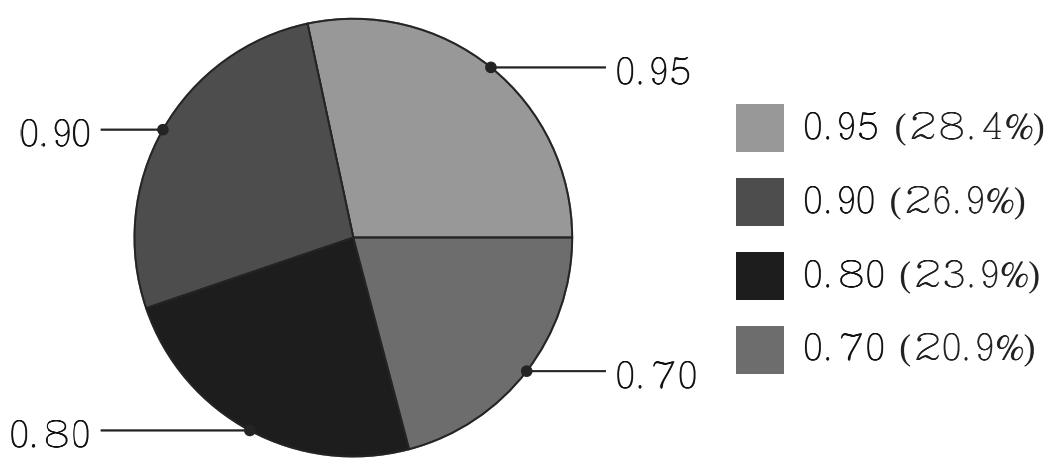
\includegraphics[width=.45\textwidth]{piechart-4weighted.png}
}
\subfigure[This one is on the right]{
\label{fig:piecharts:right}
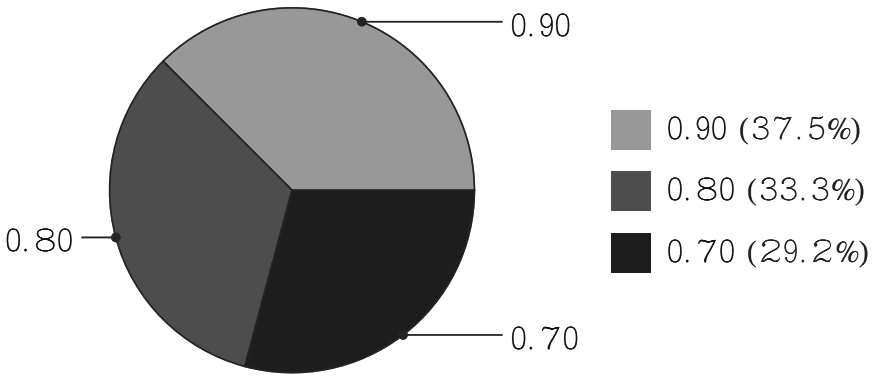
\includegraphics[width=.45\textwidth]{piechart-3weighted.png}
}
\caption{A description of the figure}
\label{fig:piecharts}
\end{center}
\end{figure} 



\chapter{ANOTHER CHAPTER}

We can also do some math!

$$fitness = F1 =\frac{2}{\frac{1}{recall} + \frac{1}{precision}}$$



And then talk about it inline: $precision =\frac{true positives}{true positives
+ false positives}$

\subsection{Some method}


There is a method presented in Algorithm
\ref{alg:randomcrossover}, it is identified by reference.

\begin{algorithm}[h]
\LinesNumbered
\caption{Perform Random Crossover  $v \bigotimes u$}
\label{alg:randomcrossover}
%\SetLine
\KwIn{$v$ : Feature Subset Vector  \\
\hspace{37pt} $u$ : Feature Subset Vector }
\KwOut{$z$ : Feature Subset Vector }

\For{$0 \leq i <$ number of possible features}{
	\eIf{$0.5 < Random(0, 1)$}
		{$z[i] \leftarrow v[i]$}
		{$z[i] \leftarrow u[i]$}
	
}
\end{algorithm}





















\chapter{TABLES}
Lets make a table that will show up on the list of tables. Shown in Table
\ref{tab:complexity}


\begin{table}[h]
\begin{center}
\begin{tabular}{|c|c|}
\hline
Method & Complexity \\
\hline
\hline
GRS & $O(ic\Gamma)$ \\
\hline
WRS & $O(ic\Gamma^2)$ \\
\hline
WRSAS & $O(ic\Gamma^2)$ \\
\hline
SCCS & $O(i'rc\Gamma^2)$ \\
\hline
\end{tabular}
\end{center}

\caption{The complexity of the algorithms presented.  }
\label{tab:complexity}
\end{table}




\section*{Acknowledgment}
This research was supported in part by \ldots



\bibliographystyle{umbthes} 
\bibliography{citations}

\end {document}
